%\documentclass[12pt, preprint,numberedappendix]{emulateapj}
%\documentclass[12pt, preprint]{aastex}
%\documentclass[apj]{emulateapj}
\documentclass[12pt, letterpaper]{article}

%\newcommand\submitms{n}		% set to y to follow AAS ``ms'' names, etc.
%\newcommand\bibinc{n}		% set to y if bib pasted in .tex, set to n to use bibtex


%\usepackage{pdfsync}
%\usepackage{subeqnarray}
\usepackage[top=0.9in, bottom=0.6in, left=1in, right=1in]{geometry}
\usepackage{natbib}
\usepackage{color}
\usepackage{graphicx}
\usepackage{fancyhdr}
\usepackage[T1]{fontenc}
\usepackage{titling}
\usepackage{sectsty}
\usepackage{sidecap}
\usepackage{placeins}
\usepackage{indentfirst}
\usepackage{wrapfig}
\usepackage[font={footnotesize}]{caption}
\usepackage{multicol}
\setlength{\droptitle}{-7em}
\setlength{\abovecaptionskip}{-2.5ex}
\setlength{\belowcaptionskip}{-2.5ex}
%\pagenumbering{gobble}
\pagestyle{fancy}
\lhead{Ana-Maria Piso}
\rhead{Hubble Fellowship Previous and Current Research Statement}
\date{}
%\rhead{\thepage}


%\bibliographystyle{apj}

\title{\Large Hubble Fellowship Previous and Current Research Statement: \\
Giant Planet Formation and Snowlines in Protoplanetary Disks\vspace{-2ex}}
\author{Ana-Maria Piso \vspace{-2ex}}

%\newenvironment{packed_item}{
%\begin{itemize}
%  \setlength{\itemsep}{1pt}
%  \setlength{\parskip}{0pt}
%  \setlength{\parsep}{0pt}
%}{\end{itemize}}

\begin{document}
\maketitle

%\slugcomment{Draft Modified \today}

\vspace{-1.5cm}


Planets are born in protoplanetary disks, which means that their structure and composition are determined by and highly connected to the chemical composition and structure of the disk in which they form. In my current and previous research, I have approached this intricate disk-planet link from two directions: (1) by exploring the core accretion mechanism, specifically calculating the minimum required core mass to form a gas giant before the dissipation of the gas in the protoplanetary disk, and (2) by understanding how disk chemistry and dynamics shape the snowline locations of volatiles in disks, which has direct implications for the chemical composition of extrasolar planet (exoplanet) atmospheres. \\
\underline{\textbf{1. Minimum Core Masses for Giant Planet Formation}}

Gas giants are widely believed to form through core accretion $[1]$, a theory in which solid protoplanetary cores grow large enough to accumulate a massive atmosphere. In this model, planetesimals in a disk grow larger through collisions, eventually forming a planetary embryo, which continues to grow by attracting planetesimals in its neighborhood. Once an embryo becomes large enough so that its escape velocity exceeds the thermal velocity of the nebular gas in its vicinity, it starts accumulating a gaseous envelope. From this point on, the accretion of gas is regulated by the pressure support within the envelope --- the amount of gas a core can accumulate is limited by the atmosphere's ability to radiate away the energy due to the incoming planetesimals, as well as by envelope contraction.  



Core accretion is particularly challenging in the outer parts of a disk, where long dynamical times make it difficult for a core to grow fast enough before the gas disk dissipates on a timescale of a few million years. At the same time, however, giant planets on wide orbits have been discovered in recent years, such as the HR 8799 system $[2]$. This poses an intriguing question: how did these planets form? I addressed this issue in two papers, $[3]$ and $[4]$. Specifically, I answered the following question: what is the lowest possible core mass required to form a gas giant before disk dissipation? This minimum core mass applies when  solid cores no longer accrete planetesimals, as this would heat the gaseous envelope and inhibit the atmosphere's ability to cool and contract . Most state-of-the-art models, however, assume that a giant planet's core and atmosphere grow simultaneously ($[5]$, $[6]$), and thus have not been constructed to effectively explore the value of the true minimum core mass required to form a gas giant. We start investigating this minimum (critical) core mass $M_{\rm crit}$ in $[3]$, where we develop a core accretion model which assumes that planetesimal accretion is negligible, and instead the envelope accretes gas while undergoing Kelvin-Helmholtz contraction. 
%This gives a lower limit on the minimum (critical) core mass, Mcrit, to form a giant planet, since additional planetesimal accretion in this stage would heat up the atmosphere, inhibit its ability to cool, thus increasing the critical core mass. Moreover, while Mcrit has been systematically computed as a function of disk properties and stellocentric separation for steady-state atmospheres heated by planetesimal accretion (Rafikov 2006), no equivalent systematic study is available for this minimum value of Mcrit. 
We consider envelopes accreting around fully formed cores at distances between 5 and 100 astronomical units (AU) from their host star. We use a simple model that assumes the nebular gas to be ideal and polytropic, and that the dust opacity is the standard interstellar opacity (ISM; $[7]$). We find $M_{\rm crit}$ to decrease between 8.5 Earth Masses ($M_{\oplus}$) at 5 AU to 3.5 $M_{\oplus}$ at 100 AU. 
%These results are lower than those of standard studies, which typically assume $M_{\rm crit} \sim 10 M_{\oplus}$. 
%(Stevenson 1982). Our study hence makes great strides in understanding the formation of giant planets at large separations. Moreover, 
We note that our numerical technique has been used by $[8]$ and $[9]$ to understand planet formation in the inner disk. 

The simplified model developed in $[3]$ assumes an ideal equation of state (EOS) and an ISM opacity. To obtain more robust quantitative results for $M_{\rm crit}$, we expand this model in $[4]$ by making two important additions: (1) a realistic EOS, and (2) realistic dust opacities. We use the $[10]$ EOS tables, and we extend them to lower temperatures and pressures as suitable for the parameter space we are exploring. Moreover, we use realistic opacity tables that take into account grain growth $[11]$ to calculate $M_{\rm crit}$. We find that a realistic EOS increases $M_{\rm crit}$, while grain growth opacities, in contrast, decrease $M_{\rm crit}$. Taking these two competing effects together, we calculate $M_{\rm crit} \sim 8 M_{\oplus}$ at 5 AU, decreasing to 5 $M_{\oplus}$ at 100 AU (Figure 1). Our results are still lower than 10 $M_{\oplus}$, the typically quoted value, and may be up to one order of magnitude lower if grain coagulation is taken into account (see $[4]$ for details). Thus our studies clearly challenge previous claims that core accretion cannot operate in the outer parts of protoplanetary disks, reopening the case for in situ formation of wide-separation gas giants. 
\begin{wrapfigure}{r}{0.4\textwidth}
  \begin{center}
    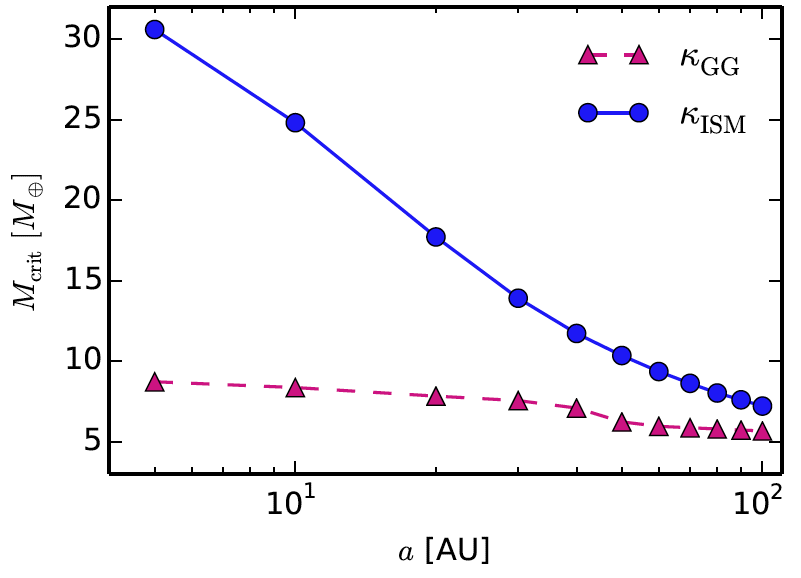
\includegraphics[width=0.4\textwidth]{Mcrit_vs_a_gg}
  \end{center}
  %\vspace{-0.1in}
  \caption{$M_{\rm crit}$ as a function of semi-major axis for a realistic EOS, and both ISM and grain growth opacities. Grain growth significantly decreases $M_{\rm crit}$ (from $[4]$).}
  %\vspace{-0.3in}
\end{wrapfigure}
\underline{\textbf{2. Snowline Locations in Protoplanetary Disks}}

The locations of volatile snowlines in protoplanetary disks are a defining feature of both gas giant and disk chemistry, as they provide vital information about the abundance of these molecules in gas and dust throughout the disk. In this part of my dissertation and beyond, I want to understand the disk well enough to (1) predict what kind of planet compositions result from planet formation in different parts of the disk, and (2) back-track the planet formation location based on planet composition. While disk structure is very complex, we do have valuable observational evidence of molecular abundance detections in disks $[12]$, as well as volatile snowlines ($[13]$, $[14]$). \\
\underline{\textbf{A. H$_2$O, CO$_2$, CO Snowlines and the C/O ratio.}} 

One important signature of disk and exoplanet chemistry is the carbon-to-oxygen (C/O) ratio, as small variations of the C/O ratio may affect the abundance of other volatiles by several orders of magnitudes (e.g., $[15]$ for the case of exoplanet atmospheres). Specifically, an important consequence of volatile condensation and sublimation in disks is that disks are expected to present different C/O ratios in the gas and in the icy dust mantles at different disk radii. This effect was quantified by $[16]$, who considered the fact that the main carriers of carbon and oxygen, i.e. H$_2$O, CO$_2$ and CO, have different condensation temperatures. This changes the relative abundance of C and O in gaseous and solid form as a function of the snowline location of the volatiles mentioned above. 

In $[17]$, we expand this model to include the effect of radial drift of solids and viscous gas accretion on the volatile snowline locations. We use a simple, semi-analytical model to solve for the coupled drift-desorption equations for particles of different initial sizes, as well as for various disk models (irradiated, evolving, viscous). For all disks, we find that particles within an initial size range desorb at a size-dependent location in the disk, which is independent of the particle's initial position. From this, we can estimate upper limits for the C/O ratio in disks (Figure 2). %The largest desorbing particles in our model have initial sizes of ~7 m, and they are representative for the snowline locations, as realistic grain size distributions are dominated in mass by the largest particles. 
By comparing the innermost snowlines in Figure 2, which are set by the largest desorbing particles ($\sim$7 m in our model), we obtain a very powerful result: radial drift and gas accretion may move the H$_2$O, CO$_2$ and CO snowlines by up to 40-60\% compared to a static disk. For a transition disk, i.e. a disk with an inner cavity significantly depleted of gas, we find that H$_2$O particles that start at an initial distance interior to the gap drift towards the original snowline, while grains located exterior to the gap stop shortly after crossing the gap edge, due to the decrease in gas pressure inside the cavity. This is qualitatively consistent with the observations of $[14]$, which show that the H$_2$O snowline is pushed outwards in a transition disk compared to a full disk. Our model framework is thus generally valid for more complicated disk structures as well. We plan to expand this model by adding several disk processes, such as turbulent diffusion, particle composition and grain morphology.
\begin{wrapfigure}{r}{0.45\textwidth}
  \begin{center}
    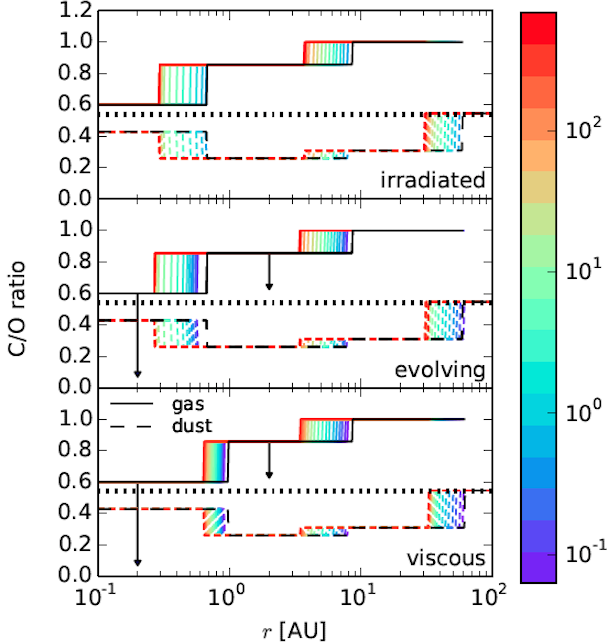
\includegraphics[width=0.46\textwidth]{C_O_ratio_passive_active_disk_many_colorbar_complete_new2}
  \end{center}
  %\vspace{-0.1in}
  \caption{Snowline locations and C/O ratios upper limits in three disk models. The color bar corresponds to the initial particle size in cm. Compared to a static disk (black lines), radial drift and gas accretion may push the snowlines inwards by 40-60\%. The arrows show that the C/O ratio in gas will decrease inside the H$_2$O and CO$_2$ snowlines in disks that take into account gas accretion, as the relative fluxes of the desorbed icy particles and the overall nebular gas will cause an excess of oxygen gas inside these snowlines (from $[17]$).}
  \vspace{-0.1in}
\end{wrapfigure}
%\vspace{-0.05in}
\underline{\textbf{B. Nitrogen Abundance and Ice Binding Energies}}

Aside from the main C and O carriers, nitrogen (N) bearing species are important to study. Nitrogen is highly abundant in the Solar system $[18]$ and disks, and primarily found as N$_2$. Because of the high volatility of N$_2$, the gas phase nitrogen-to-oxygen (N/O) ratio in the outer disk may be even more enhanced than the C/O ratio. Giant planets that form at wide separations should thus have an excess of N in their atmospheres, which could be used to trace their formation origin. In $[19]$, we quantify this effect in disks. We find that the N/O ratio in gas is significantly larger than the Solar abundance, and indeed exceeds the C/O ratio in the outer disk. We can thus set the stage to answer one of our main questions, i.e. back-track the planet formation location based on planet composition. In this study we also explore the effects of assuming that N$_2$ is bound to water ice instead of pure N$_2$, and the presence of some N in the form of NH$_3$. In either case, the general result of a large N/O enhancement in the outer disk is preserved. \\
\underline{\textbf{C. Self-consistent C/N/O Calculation}}

As shown in Figure 2, our current drift-desorption model can only provide us with upper estimates for C/O (or N/O) ratios. We plan to enhance this model by performing the time-dependent calculation that accounts for the relative motion of the desorbed ices and the overall nebular gas, the time evolution of the dust surface density,  and radial gas diffusion; all these effects will change the volatile abundances and the C/O ratio in time. We have developed a code that evolves the dust surface density for a particle of fixed size. Next, we will treat  each species in gaseous and solid forms as two fluids that are interchanging. Following $[20]$, we will use advection-like equations to solve for their separate time-dependent abundance.



%\begin{figure}[h!]
%\centering
%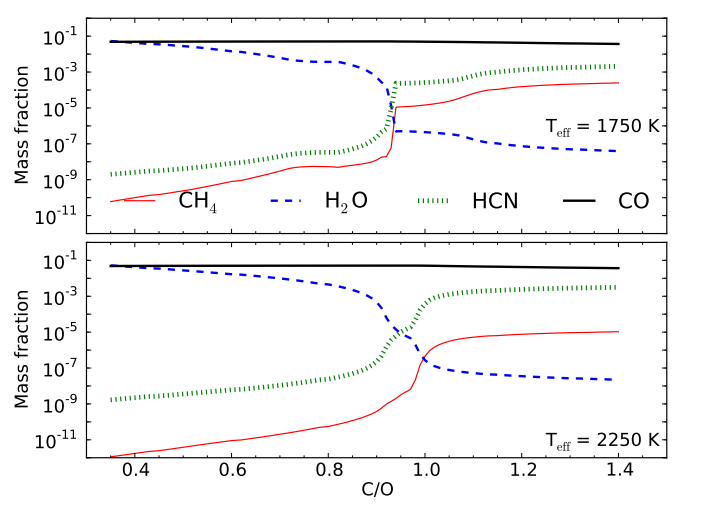
\includegraphics[width=0.7\textwidth]{CO_abundances}
%%\vspace{-0.5in}
%\caption{TBD}
%\label{fig:CO}
%\end{figure}


%\if\bibinc n
%\bibliography{refs}
%\fi
%\FloatBarrier
%\def\bibfont{\footnotesize}
%\setlength{\bibsep}{0.0pt}

\footnotesize

%\textbf{References} \\
%\begin{thebibliography} {9}
\begin{multicols}{2}
\noindent 
$[1]$ Pollack, et al. 1996, Icarus, 124, 62 \\
$[2]$ Marois, C.,  et al.. 2008, Science, 322, 1348 \\
$[3]$ \textbf{Piso, A.-M. A.},\&Youdin,A.N. 2014,ApJ,786,21 \\
$[4]$ \textbf{Piso, A.-M. A.}, et al. 2015, ApJ, 800, 82 \\
$[5]$ Bodenheimer, P.\&Pollack, J. 1986, Icarus, 67, 391 \\
$[6]$ Rafikov, R. R. 2006, ApJ, 648, 666 \\
$[7]$ Bell, K. R. \& Lin, D. N. C. 1994, ApJ, 427, 987 \\
$[8]$ Lee, E. J., et al. 2014, ApJ, 797, 95 \\ 
$[9]$ Lee, E. J., \& Chiang, E. 2015, ApJ, 811, 41 \\
$[10]$ Saumon, et al. 1995, ApJS, 99, 713 \\
$[11]$ D'Alessio, P., et al. 2001, ApJ, 553, 321 \\
$[12]$ Henning,T.,\&Semenov, D. 2013, ChRv, 113, 9016 \\
$[13]$ Qi, C., et al. 2013, Science, 341, 630 \\
$[14]$ Zhang, K., et al. 2013, ApJ, 766, 82 \\
$[15]$ Molli{\`e}re, P., et al. 2015, ApJ, 813, 1 \\
$[16]$ \"Oberg, K. I., et al. 2011, ApJ, 743, L16 \\
$[17]$ \textbf{Piso, A.-M. A.}, et al. ApJ (under review) \\
$[18]$ Lodders, K. 2009, arXiv:0910.0811 \\
$[19]$ \textbf{Piso, A.-M. A.}, et al. (in prep) \\
$[20]$ Ciesla, F. J. \& Cuzzi, J. N. 2006, Icarus, 181, 178


%Stevenson, D. J. 1982, Planet. Space Sci., 30, 755 \\

\end{multicols}
%\end{thebibliography}

%\bibliographystyle{abbrv}
%\bibliography{refs}


%\if\bibinc y
%\begin{thebibliography}
%\end{thebibliography}
%\fi


\end{document}